\section{Rendering the Game}

One very important aspect of the client program is rendering the current game state to a display for the user to interact with. Creating a picture of the game to display requires a number of graphical assets to visually represent the various entities and scenery that make up the game world. For Project Serenity all of these graphics were created from scratch using Photoshop and Illustrator. Figure~\ref{fig:textures} shows a selection of some of the assets that were created for different entities.

\begin{figure*}[h!]
	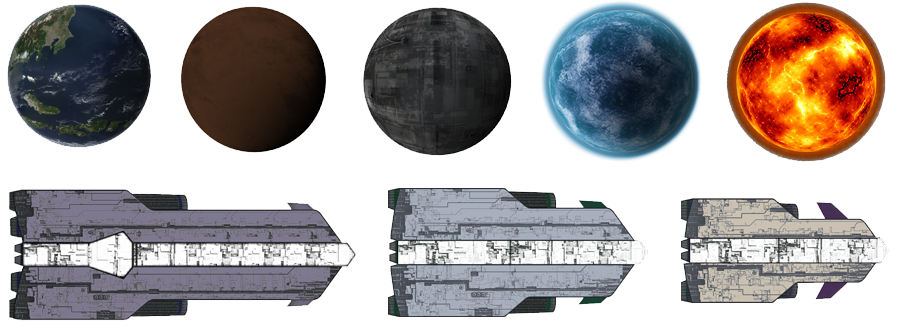
\includegraphics{res/serenityscreens/textures.png}
	\caption[Planet and ship textures created for Project Serenity][1em]{Planet and ship textures created for Project Serenity.}
	\label{fig:textures}
\end{figure*}

The client uses these assets to draw the sector and place each player's ships in the correct locations. This is done by placing the assets using world coordinates in the 2D space defined by the dimensions of the sector. The picture that has been built up so far is then translated and scaled according to the current panning and zoom settings stored in the client. This allows the user to smoothly zoom in and out as well as scroll around the sector. There are optimisations that could have been performed, such as working out which entities would be displayed and only drawing them instead of drawing them and scaling them out of view, but in the end there were not required.

\begin{figure*}[p]
	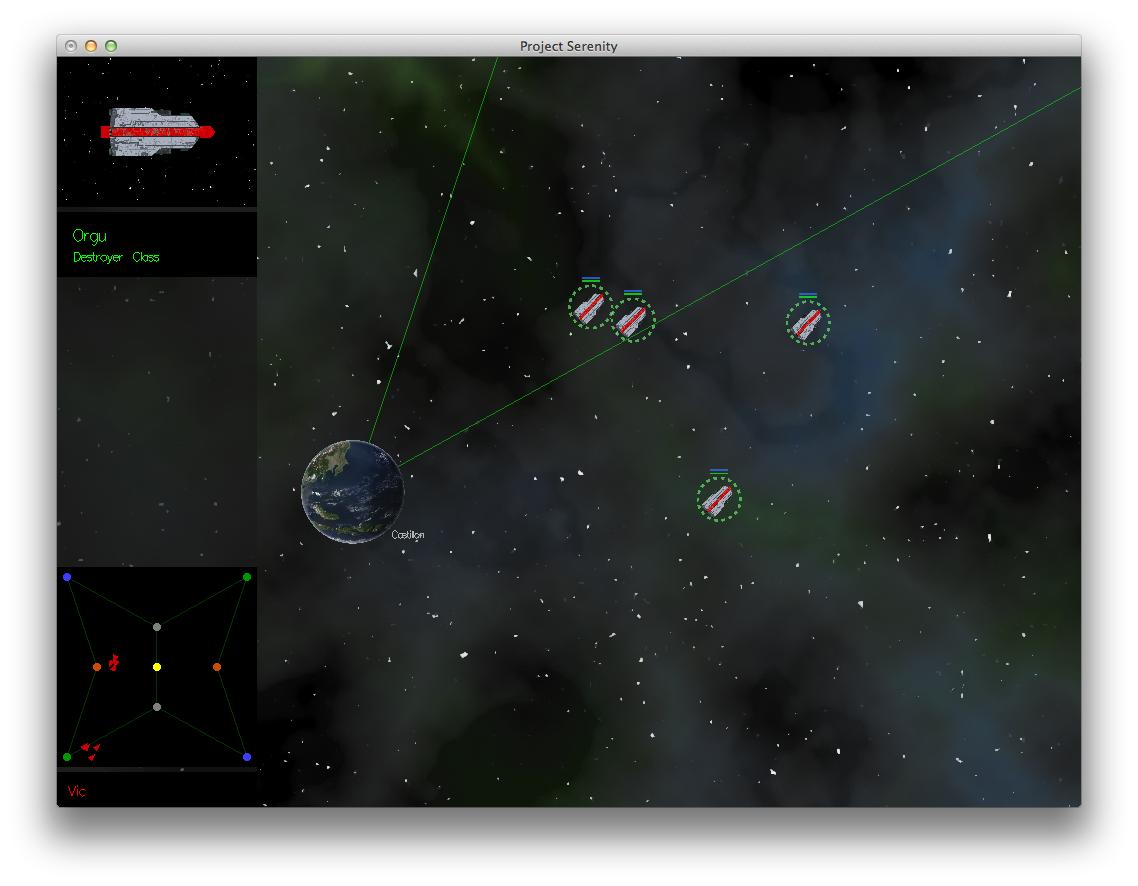
\includegraphics[width=15.5cm]{res/serenityscreens/09-ingame1}
	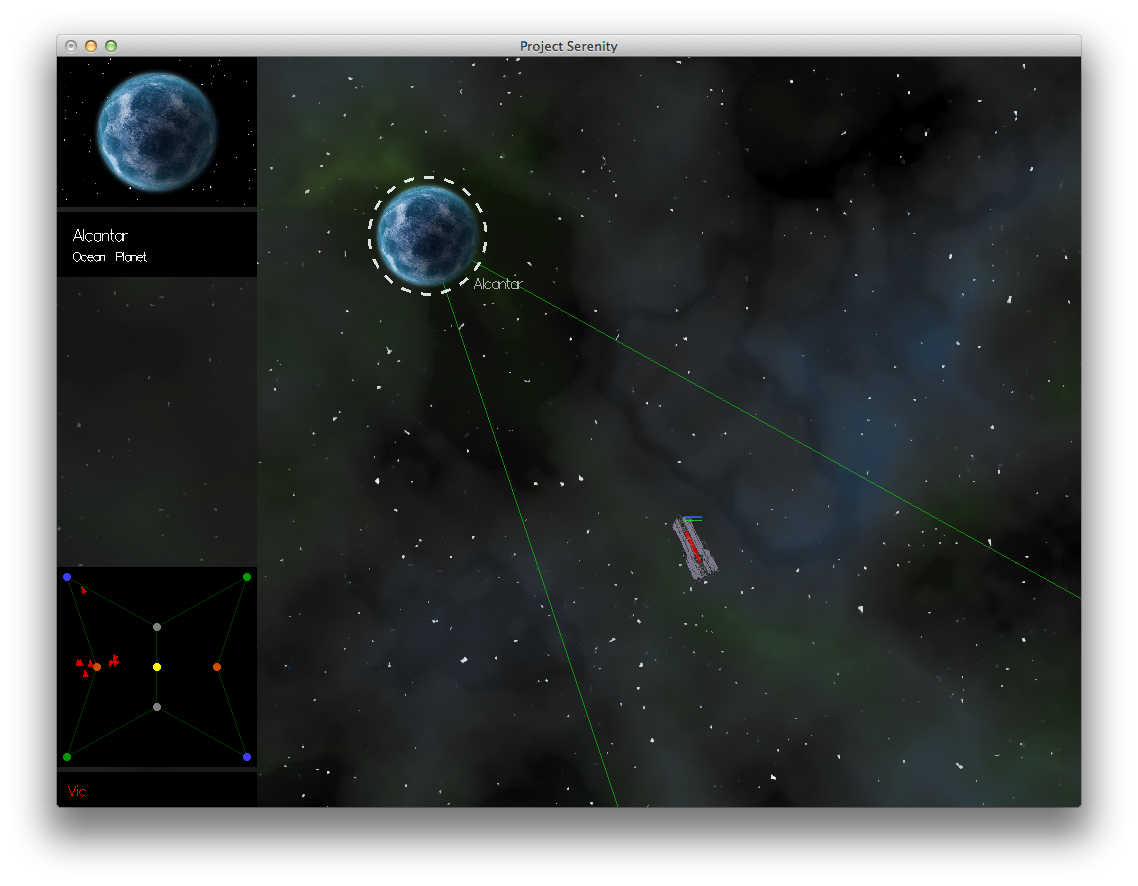
\includegraphics[width=15.5cm]{res/serenityscreens/10-ingame2}
	\caption{Screenshot during gameplay showing a planet, spacelanes, selected ships, and minimap.}
	\label{fig:gameplay}
\end{figure*}

Along with the actual world there is some extra GUI elements to help the player keep track of the current state of the game. Firstly there is a minimap in the bottom left corner. This displays a schematic representation of the sector with the locations of friendly ships. The minimap allows the user to quickly check on the current status of their fleet. It was originally hoped that the minimap could be used to show extra events such as known locations of enemies and current attacks. It could also be enhanced by allowing the user's view to be transported to the location clicked on the minimap. However, core features were prioritised over this extra functionality, and so they are not implemented yet.

The second piece of GUI is the ship and planet selection indicators. When a user left clicks on an entity, or drags a selection box over a group of entities, they are selected and a dashed selection circle surrounds the entity. To make this feature easier to use a group selection does not select all entities within the drag area. Instead some are prioritised over others: ships are ranked above planets, and friendly ships are ranked above enemies. For example, if a selection is made over the entire sector then only the friendly ships will be selected. If a single entity is selected then details about it will be shown in the top left of the screen.

Figure~\ref{fig:gameplay} shows how similar the resulting game was to the initial mockup made during the specification stage (see Figure~\ref{fig:mockup1}).

% TODO Talk about parallax because it's interesting? (Innovative?)

Another interesting piece of the rendering puzzle was to choose a colour as a unique visual representation for each player. This would be used to help players differentiate their ships from the enemy and to identify the planets that they own. A clever algorithm was used that would take a numerical player identifier and return a unique colour:\cite{ankerl2009}

\begin{equation*}
	colour(i) = HSV(i \times \phi^{-1} \mod 1, 1.0, 0.8)
\end{equation*}
\noindent
This function uses the HSV colour space using a fixed saturation and value, but modifying the hue to create equally bright and vibrant colours. The player's identifier, $i$, is used to step into the possible values for hue by multiplying it by the reciprocal of the golden ratio, $\phi$, modulo one. Due to the equidistribution theorem\sidenote{The equidistribution theorem states that the sequence $a, 2a, 3a, \ldots \mod 1$ is uniformly distributed when $a$ is an irrational number} this creates a sequence of colours that are evenly spread across the colour space. Using this method to generate team colours created visually pleasing colours that are suitably distinct from each other to be used for recognition.
